\documentclass[fleqn]{article}
\usepackage{ctex}
%\usepackage{xeCJK}
%\setCJKmainfont{AR PL UMing TW MBE}
%\setCJKmainfont{FangSong_GB2312}
\usepackage[breaklinks,colorlinks,linkcolor=black,citecolor=black,urlcolor=black]{hyperref}
\newcommand{\tabincell}[2]{\begin{tabular}{@{}#1@{}}#2\end{tabular}}  
\begin{document}
\title{高数学习}
\author{韩海舰}
\maketitle
\setlength{\mathindent}{10pt}
\begin{flushleft}
高等数学上(mooc课程学习笔记,深圳大学)
\section{第一章\quad 函数,极限,连续性}
\subsection{第一周练习}
1.已知f(x+1)的定义域为[0,a](a>0),则f(x)的定义域为()。
\begin{enumerate}
\item $[1,a+1]$
\item $[-1,a+1]$
\item $[a,a+1]$
\item $[a-1,a]$
\end{enumerate}

正确答案:A你错选为B

2. \[\texttt{若}\lim_{n\to \infty}x_n=a\texttt{(a为常数),则下列说法不正确的是。}\]
\begin{enumerate}
\item 数列$\{x_n\}$有界。
\item \[\lim_{n\to \infty}x_{2n}=a\]
\item 若$x_n>0$(n=1,2...n),则a>0
\item 常数a唯一。
\end{enumerate}
正确答案:C你没选择任何选项

极限的性质包括:唯一性,有界性,保号性。其中保号性是指如果极限>0,则$x_n$>0。
\subsection{第二周练习}
\par
1.已知函数\[
f(x)=\left\{\begin{array}{ll}
x^2sin\frac{1}{x} ,& x<0 \\
\frac{\sqrt{1+x^2}-1}{x}, & x>0
\end{array}
\right. 
\]
\[\texttt{则}\lim_{x\to 0}f(x)=(?)
\]
结果为0
\par
2.\[
\texttt{若}\lim_{x\to 0}f(x)=0,\texttt{则()}\]
\begin{enumerate}
\item \[\texttt{仅当}\lim_{x\to x_0}g(x)=0\texttt{时,才有}\lim_{x\to x_0}f(x)g(x)=0\texttt{成立。}\]
\item \[\texttt{当}g(x)\texttt{为任意函数时,有}\lim_{x\to x_0}f(x)g(x)=0\texttt{成立}\]
\item \[\texttt{仅当}g(x)\texttt{为常数时,才能使}\lim_{x\to x_0}f(x)g(x)=0\texttt{成立}\]
\item \[\texttt{当}g(x)\texttt{有界时,能使}\lim_{x\to x_0}f(x)g(x)=0\texttt{成立}\]
\end{enumerate}
答案是4.\[\lim_{x\to 0}f(x)=0\]是无穷小,无穷小与有界函数之积是无穷小。

3.\[
\lim_{x\to 0}(1-x)^{\frac{1}{sinx}}=(?)\]
\begin{enumerate}
\item 1
\item e
\item $e^{-1}$
\item $e^{-2}$
\end{enumerate}

正确答案:C你错选为B


\subsection{第三周练习}
等价无穷小:
\begin{equation}
\begin{array}{|ll|}
\hline
sin(x) \sim x ,& tan(x) \sim x\\
arcsin(x) \sim x &\\
e^x-1 \sim x, & a^x -1 \sim x\ln a\\
\ln(x+1)\sim x ,& 1-cos(x) \sim \frac{1}{2}x^2\\
\sqrt[n]{1+x}-1 \sim \frac{1}{n}x\\
\hline
\end{array}
\end{equation}
有用极限:
\begin{equation}
\begin{array}{|l|}
\hline
\lim_{x\to 0}(1+x)^{\frac{1}{x}}=e\\
\hline
\end{array}
\end{equation}

无穷小的关系:
\[
\alpha =lim{f(x)}=0,\beta =\lim{g(x)}=0,\texttt{均是无穷小}
\]
\[
\begin{array}{|l|l|l|}
\hline
\texttt{高阶无穷小:}&\frac{\alpha}{\beta}=0&\alpha\texttt{是}\beta\texttt{的高阶无穷小}\\
\hline
\texttt{等价无穷小:}&\frac{\alpha}{\beta}=1&\alpha\texttt{是}\beta\texttt{的等阶无穷小}\\
\hline
\texttt{同价无穷小:}&\frac{\alpha}{\beta}=c\quad(c\neq 0)&\alpha\texttt{是}\beta\texttt{的同阶无穷小}\\
\hline
\texttt{k价无穷小:}&\frac{\alpha}{\beta^k}=c\quad(c\neq 0)&\alpha\texttt{是}\beta\texttt{的k阶无穷小}\\
\hline
\end{array}
\]
\paragraph
\indent matlab中求极限\\
\begin{verbatim}
limit(f,x,a)
f是表达式,可以直接用'xxx',也可用syms来定义。
x表示自变量,a表示趋向。
例如:
limit('(exp(x)+exp(-x))/sin(x)',x,0)
or
syms x y;
y=(exp(x)+exp(-x))/sin(x);
limit(y,x,0)
结果为2
\end{verbatim}


\section{导数与微分}
\subsection{第四周练习}
1.设函数f(u)可导,且$y=f(x^2)$当自变量x在x=1处取得增量$\Delta x=-0.1$时,相应的函数增量$\Delta y$的线性主部为0.1,则$f^{'}(1)=().$
\begin{enumerate}
\item 0.1
\item 1
\item -0.5
\item -1
\end{enumerate}
正确答案:C你错选为D

2.函数y=f(x)在$x_0$处连续、可导、可微的关系中不正确的是:
\begin{enumerate}
\item 可导是可微的充分必要条件
\item 可微是连续的充分条件
\item 连续是可导的充分必要条件
\item 连续式可微的必要条件
\end{enumerate}
正确答案:C你错选为A
\par
连续:
\begin{enumerate}
\item f(x)在$x_0$处有定义
\item f(x)在$x_0$处有极限
\item \[\lim_{x\to x0}f(x)=f(x0)\]
\end{enumerate}
可导:
\begin{enumerate}
\item f(x)在$x_0$的邻域内有定义
\item \[\lim_{\Delta x\to 0}\frac{\Delta y}{\Delta x}=\lim_{\Delta x\to 0}\frac{f(x0+\Delta x)-f(x_0)}{\Delta x}\]存在
\item \[f_{+}^{'}(x_0)=f_{-}^{'}(x_0)\]
\end{enumerate}
可导$\Longrightarrow$连续,但连续未必可导。可导
$\Longleftrightarrow$可微

二阶导数:\[\frac{d^2y}{dx^2}=\frac{d\frac{dy}{dx}}{dx}\]

\section{第三章微分中值定理与导数应用}
\subsection{第六周练习}
1.求$\lim_{x\to 0}\left\lbrace\frac{sinx}{x}\right\rbrace^\frac{1}{1-cosx}=()$
\begin{enumerate}
\item 1
\item $e^{-\frac{1}{3}}$
\item $e^{\frac{1}{6}}$
\item $e^2$
\end{enumerate}
正确答案:B你错选为A
\paragraph
2.求$lim_{x\to 1}\left\lbrace\frac{3}{1-x^3}-\frac{1}{1-x}\right\rbrace=()$
\begin{enumerate}
\item -1
\item 0
\item $\infty$
\item $1$
\end{enumerate}
正确答案:D你错选为C\\
通分
\paragraph
3.函数$y=x^2+4x-5$在区间[-6,6]上\\
\begin{enumerate}
\item 先单调减少再单调增加
\item 先单调增加再单调减少
\item 单调增加
\item 单调减少
\end{enumerate}
正确答案:A你错选为C\\
注意x的区间,判断y'的符号

\subsection{第七周练习}
\paragraph
1.函数$y=\frac{lnx}{x}$在区间$(0,+\infty)$内,
\begin{enumerate}
\item 无极值 
\item 最大值为$\frac{1}{e}$
\item 最小值为$\frac{1}{e}$
\item 无最大值
\end{enumerate}
正确答案:B你错选为A\\
求导,x=e,
\paragraph
2.曲线$y=e^{-(x-1)^2}$的渐近线是
\begin{enumerate}
\item x=1为铅直渐近线,y=1是水平渐近线 
\item x=1为铅直渐近线,y=0是水平渐近线
\item y=0是水平渐近线
\item x=0为铅直渐近线,y=0是水平渐近线
\end{enumerate}
正确答案:C你错选为A\\
$lim_x\to \infty f(x)=?$判断水平渐近线,$lim_x\to x0 f(x)=?$判断铅直渐近线。

拐点:凹凸转折点。\\
拐点的充分必要条件:f(x)在(a,b)内二阶可导,$f^{''}(x_0)=0,x_0\in{(a,b)}$,而且$f^{''}(x_0)$处两边符号不相等

\paragraph
曲率:反应曲线的弯曲程度。直线的曲率为0,圆的曲率为1/R.圆的半径越大,则曲率越小,否则曲率越大。
\[K=\lim_{\Delta S\to 0}\frac{\alpha}{\Delta S} \]$\alpha$是弧的转角。
曲率的计算公式:
\begin{equation}
\begin{array}{|l|}
\hline
\frac{|y^{''}|}{(1+y^{' 2})^{\frac{3}{2}}}\\
\hline
\end{array}
\end{equation}
\begin{verbatim}
matlab中的函数
定义符号:syms x
求导:diff(f)
例如:f=sin(x);diff(f);
积分:
符号积分:
int(fun,x)计算不定积分
int(fun,x,a,b):计算定积分
例如:
f=sinx;int(f)
int(f,-pi,pi);

数值积分:
trapz(x,y):梯形积分
例如:x=-1:0.01:1
y=tan(x);
trapz(x,y);

quad(fun,x,a,b)辛普森积分
fun可以是匿名函数@(x),或内联函数inline()
比如y=cosx,可以表示成:
y=@(x)cos(x)
y=inline('cos(x)')
例如:
y=@(x)tan(x)
quad(y,-1,1)

pretty(fx)人性化显示公式
\end{verbatim}

\section{第四章 一元函数积分学}
\subsection{第九周练习}
1.f(x)在[a,b]上连续是$\int_a^b{f(x)dx}$的()
\begin{enumerate}
\item 充分必要条件
\item 必要非充分条件
\item 既非充分也非必要条件
\item 充分而非必要条件
\end{enumerate}
正确答案:D你错选为C
\paragraph
若f(x)在[a,b]连续,则其上界函数$\int_a^xf(t)dt$必然是其原函数,即函数连续必有原函数。


\paragraph
2.求$\int \frac{\sqrt{x^2-9}}{x^2}dx$\\
正确答案:$ln|x+\sqrt{x^2-9}|-\frac{1}{x}\sqrt{x^2-9}+C$
\paragraph
3. 求$\int_a^bf(mx+n)dx=$\\
正确答案:$\frac{1}{m}\int_{ma+n}^{mb+n}f(x)ds$
\paragraph
4 求 $\int_0 ^{1/2} \frac{x^2}{\sqrt{1-x^2}}dx$\\
正确答案:$\pi/12-\sqrt{3}/8$
\paragraph
5求$\int_{-2}^{2}(e^{x^2}sinx^3-\sqrt{4-x^2})dx$\\
正确答案:$-2\pi$

\subsection{第十一周练习}
\paragraph
1.求$\int(x^2+1)e^{2x}dx$\\
正确答案:$\frac{1}{2}(x^2+1)e^{2x}-\frac{1}{2}xe^{2x}-\frac{1}{4}e^{2x}+C$

\paragraph
2.已知f(x)的原函数是$tan^2x$,则$\int_0^1 xf^{'}(x)dx=?$\\
答案是:$2tan1sec^21+tan^21$

\paragraph
3.求$\int_{\frac{-1}{2}}^{\frac{1}{2}}\frac{xarcsinx}{\sqrt{1-x^2}}dx$\\
答案是:$1-\frac{\sqrt{3}}{6}\pi$
\paragraph
4.求$\int_{-1}^{2}\frac{1}{x^2}dx$\\
答案是发散。由于积分区间中存在瑕点。

\section{第五章积分应用}
\subsection{第十二周练习}
\paragraph
1.计算心形$\rho=1+cos\theta$和圆$\rho=3cos\theta$所围公共部分面积。\\
正确答案:$5\pi/4$
\paragraph
2.已知一弹簧原长1米,把它压缩1厘米所用的力为0.05牛顿,把弹簧从80厘米压缩到60厘米所做的功()\\
正确答案:0.3(N.m)
\paragraph{}
\begin{tabular}{|l|}
\hline
计算曲线面积\\
直角坐标:$ds=y*dx$\\
极坐标:$ds=\frac{\rho^2 d\theta}{2}$\\
\\
计算曲线长度:\\
直角坐标:$ds=\sqrt{1+y^{'2}}dx$\\
参数方程:$ds=\sqrt{dx^2(t)+dy^2(t)}$\\
极坐标:$ds=\sqrt{\rho^2+\rho^{' 2}}d\theta$\\
\hline
\end{tabular}

\paragraph{}
\textbf{常用积分公式}
\begin{equation}
\begin{array}{|l|}
\hline
\int lnxdx=xlnx-x+C\\
\int sin^2 xdx=\frac{x}{2}-\frac{sin2x}{4}+C \\
\\
\int cos^2 xdx=\frac{x}{2}+\frac{sin2x}{4}+C\\
\\
\int cos^m x sin^n xdx=\frac{1}{m+n}cos^{m-1} x sin^{n+1}x +\frac{m-1}{m+n}\int cos^{m-2}x sin^{n}x+C
\\
\hline
\end{array}
\end{equation}
\section{第六章\quad 微分方程}
\subsection{第十三周练习}
1.微分方程$\frac{dy}{dx}=2x$的一条积分曲线与直线$y=2x+3$相切,则切点为:\\
正确答案:(1,5)\\

直线斜率为2,积分曲线切线斜率为y'=2x,$2x=2\Longrightarrow x=1 \Longrightarrow y=5$
\paragraph
2.微分方程$xy'+y=y(lnx+lny)$的通解为:\\
正确答案:$y=\frac{1}{x}e^{Cx}$\\
用换元法,u=xy
\paragraph
3.设y(x)满足微分方程$xy'+y-y^2lnx=0,y(1)=1,$则,y(e)=?\\
正确答案:1/2\\
用换元法,u=1/y,将方程转换成u,x的非齐次线性方程,然后用公式,最后代回。
\subsection{第十四周练习}
\paragraph
1.$y^{''}=e^{_x}$的通解为:\\
正确答案:$e^{-x}+C_1 x+C_2 $
\paragraph
2.微分方程$xy^{''}+xy^{' 2}-y{'}=0$的通解\\
正确答案:$y=ln(x^2+2C_1)+C_2$\\
化简后方程变为:$y^{''}+y^{' 2}-y^{'}/x=0$ 。符合$y^{''}=f(x,y^{'})$格式,所以用$p=y^{'}$替换,替换后变成伯努立方程,两边同除$p^2$,然后用公式。
\subsection{第十五周练习}
1.微分方程$y''+y=x+sinx$的特解是:y=()\\
\begin{enumerate}
\item $Ax+B+Ccosx+Dsinx$\\
\item $Ax+B+Cxsinx$\\
\item $Ax+B+x(Ccosx+Dsinx)$\\
\item $Ax+x(Ccosx+Dsinx)$
\end{enumerate}
正确答案C,错答为B
\paragraph
2.微分方程$y''+3y'+2y=x^2e^{-2x}$的特解是:y=()\\
\begin{enumerate}
	\item $y=ax^2e^{-2x}$\\
	\item $y=(ax^2+bx+c)e^{-2x}$\\
	\item $y=x(ax^2+bx+c)e^{-2x}$\\
	\item $y=x^2(ax^2+bx+c)e^{-2x}$
\end{enumerate}
正确答案C,错答为D\\
$\lambda=-2,m=2,\lambda_1=-2,\lambda_2=-1,k=1$

\paragraph
3.微分方程$y''-y'=e^{x}+1$的通解是:y=()\\
\begin{enumerate}
	\item $y=C_1+C_2e^x$\\
	\item $y=axe^x+b$\\
	\item $y=C_1+C_2e^x+xe^x-x$\\
	\item $y=C_1+C_2e^x-x$
\end{enumerate}
正确答案C,错答为D\\
通解为齐次方程的通解+非齐次方程的特解。齐次方程的通解为$y=C_1+C_2e^x$,特解为
$xe^x-x$

\paragraph
3.微分方程$y''+4y=1/2cos2x$的通解是:y=()\\
\begin{enumerate}
	\item $y=x(ACos2x+Bsin2x)$\\
	\item $y=Acos2x+Bsin2x+1/8xsin2x$\\
	\item $y=Acos2x+Bsin2x$\\
	\item $y=A+Be^{-4x}+1/8xcos2x$
\end{enumerate}
正确答案B,错答为C\\
通解为齐次方程的通解+非齐次方程的特解。特征根$0\pm2i$,齐次方程的通解为$y=C_1cos2x+C_2sin2x$,特解只能选B。

\paragraph
4.微分方程$y''-4y'+3y=9$的通解是:y=()\\
\begin{enumerate}
	\item $y=C_1e^x+C_2e^{3x}$\\
	\item $y=e^x(C_1cos3x+C_2sin3x)-3$\\
	\item $y=C_1e^x+C_2e^{3x}+3$\\
	\item $y=C_1e^x+C_2e^{3x}+3x^2$
\end{enumerate}
正确答案C,错答为A\\
通解为齐次方程的通解+非齐次方程的特解。特征根为1,3,齐次方程的通解为$y=C_1e^x+C_2e^{3x}$,将待选的特解带入方程只有选C。

\newpage
\paragraph
\indent 微分方程定义:含有未知函数和未知函数导数的方程称为微分方程。\\
\indent 注意不是所有含有未知函数导数的方程都是微分方程,比如u'v+uv'=(uv)'就是一个恒等式,它不是微分方程。\\
\paragraph
\indent 微分方程的分类:
\indent 导数的最高阶数称为微分方程的阶。\\
含有一个未知变量的函数,称为常微分方程;\\
含有2个以上未知变量的函数,称为偏微分方程。
\paragraph
\indent 微分方程的解:\\
微分方程的解是函数。将该函数带入原方程使得原方程恒成立,将此函数称为微分方程的解\\
含有微分方程阶数的个数个独立常数的解称为微分方程的通解。\\
不含常数的解称为微分方程的特解。\\
含有初始条件的微分方程称为初始问题。
\paragraph
\indent 一阶常微分方程:\\
\begin{tabular}{|l|l|l|}
\hline
方程名称&方程格式&方程解\\
\hline
可分离变量方程 & \tabincell{l}{$\frac{dy}{dx}=f(x)g(y)(g(y)\neq 0)$\\或$f(x)dx=g(y)dy$} &\\
\hline
齐次方程 & $\frac{dy}{dx}=f(\frac{y}{x})$ &\\
\hline
齐次线性方程 & \tabincell{l}{$\frac{dy}{dx}+p(x)y=0$\\或$y'+p(x)y=0$ }& $y=Ce^{- \int p(x)dx}$\\
\hline
非齐次线性方程 &\tabincell{l}{$\frac{dy}{dx}+p(x)y=q(x)$\\或$y'+p(x)y=q(x)$ }&\tabincell{l}{$y=e^{- \int p(x)dx}\left(\int{q(x)e^{\int{p(x)dx}}dx+C}\right)$\\或常数变量法}\\
\hline
伯努力方程 & $\frac{dy}{dx}+p(x)y=q(x)y^n,n\neq0,1$ & \tabincell{l}{两边除以$y^n$,转换成非齐次线性方程,\\然后用公式法或常数变量法求解。}\\
\hline
\end{tabular}
\paragraph
\indent 二阶微分方程\\
\noindent 可降阶的微分方程:$y^{''}=f(x,y,y^{'})$,思路是将二阶降为一阶\\
\begin{tabular}{|l|l|}
	\hline
	方程形式 & 降阶方法\\
	\hline
	$y^{''}=f(x)$ & 逐级不定积分\\
	\hline
	$y^{''}=f(x,y^{'})$ & 令 $y^{'}=p(x)$\\
	\hline
	$y^{''}=f(y,y^{'})$ & 令$y^{'} =p(y)$,$y^{''}=dp/dy*p$\\
	\hline
\end{tabular}
\paragraph
\indent 二阶线性常微分方程:
\begin{tabular}{|p{2cm}|l|l|}
	\hline 
	方程名&方程格式&解格式\\
	\hline 
	二阶齐次线性常微分方程 & $y^{''}+p(x)y^{'}+q(x)y=0$ & \tabincell{l}{$y=C_1y1+C_2y2$\\y1,y2是线性无关的解}\\
	\hline 
	二阶非齐次线性常微分方程 & $y^{''}+p(x)y^{'}+q(x)y=f(x)$ & \tabincell{l}{$y=y+Y$\\Y是对应齐次方程的通解,y是方程特解。}\\
	\hline 
\end{tabular}

\paragraph
\noindent 二阶常系数线性常微分方程:
\begin{tabular}{|p{2cm}|l|l|}
	\hline 
	方程名&方程格式&解格式\\
	\hline 
	二阶常系数齐次线性常微分方程 & $y^{''}+py^{'}+qy=0$ & \begin{tabular}{l}根据$r^2+pr+q=0$特征方程结果\\ \begin{tabular}{lll}
$p^2-4q$的结果&根&通解\\
$p^2-4q>0$ & $\lambda_1,\lambda_2$,单根&$C_1e^{\lambda_{1}x}+C_2e^{\lambda_{2}x}$\\
$p^2-4q=0$ &$\lambda$,重根 & $(C_1+x)e^\lambda x$\\
$p^2-4q<0$ & $\alpha \pm i\beta $,共轭根&$e^{\alpha x}[C_1 cos(\beta x)+C_2 sin(\beta x)]$
\end{tabular}
\end{tabular}\\
	\hline
	二阶常系数非齐次线性常微分方程 & $y^{''}+py^{'}+qy=f(x)$ & \begin{tabular}{l}\tabincell{l}{通解:$y=y+Y$\\Y是对应齐次方程的通解,y是方程特解}\\
	自由项情况1:$f(x)=e^{\lambda x}Q_m(x)$\quad $Q_m(x)$是x的m次多项式\\
	\hline
	根据特征方程$r^2+pr+q=0$根的结果和$2\lambda+p$的情况\\
	特解:$y=x^k e^{\lambda x}P_{m}(x)$,$P_m(x)$是x的m次多项式\\
	\begin{tabular}{|l|l|l|}
		\hline
		特征方程结果&k&\\
		\hline
		$\lambda^2+p\lambda+q\neq 0$ & k=0 &$\lambda$不是特征方程的根\\
		\hline
		$\lambda^2+p\lambda+q=0$和$2\lambda+p\neq 0$ & k=1 &$\lambda$是单根\\
		\hline
		$\lambda^2+p\lambda+q=0$和$2\lambda+p=0$ & k=2&$\lambda$是重根 \\
		\hline
	\end{tabular}\\
	\linebreak[2]
	自由项情况2:$f(x)=e^{\lambda x}(P_l(x)cos\omega x+P_n(x)sin\omega x)$\\
	\hline
	$P_l(x),P_n(x)$是x的l,n次多项式\\
	根据特征方程$r^2+pr+q=0$根的结果\\
	特解:$y=x^k e^{\lambda x}[R_m^{(1)} (x)cos(\omega x)+R_m^{(2)}(x)sin(\omega x)]$\\
	m=max(l,n),$R_m(x)$是关于x的m次多项式\\
	\begin{tabular}{|l|l|}
		\hline
		特征方程结果&k\\
		\hline
$\lambda+i\omega$不是特征方程的根 & k=0 \\
		\hline
$\lambda+i\omega$是特征方程的根 & k=1 \\
		\hline
	\end{tabular}
\end{tabular}\\
\hline
\end{tabular}
\newpage
\begin{verbatim}
matlab中的微分方程:
符号微分方程:
dsolve('eq1,eq2..','con1,con2','v')
eq1,eq2..微分方程,
con1,con2..初始条件,
v	变量
Dy	表示导数y'
例子:
求y'+3xy=4x的通解
syms y x;
dsolve('Dy+3*x*y=4*x','x')
ezplot(y);
ans =
 
4/3+exp(-3/2*x^2)*C1
 
 
>> pretty(ans)
 
                                             2
                            4/3 + exp(- 3/2 x ) C1
\end{verbatim}
\section{期末考试}
\paragraph
1.当$x\rightarrow 0 $时,下列哪一个无穷小时对于x的三阶无穷小()
\begin{enumerate}
		\item $x^3+0.0001x^2$
		\item $\sqrt{a+x^3}-\sqrt{a} \quad (a>0)$
		\item $\sqrt[3]{x^2}-\sqrt{x}$
		\item $\sqrt[3]{tanx}$
\end{enumerate}
正确答案B,错选A\\
高阶无穷小的概念是$lim\frac{\alpha}{\beta^k}=C,C\neq0$,只有\\
$lim\frac{\sqrt{a+x^3}-\sqrt{a}}{x^3}=C$,所以选B。


\paragraph
2.$\int{xf''(x)dx=()}$
\begin{enumerate}
		\item $xf(x)-\int{f(x)dx}$
		\item $xf''(x)-xf'(x)-f(x)+C$
		\item $xf'(x)+f(x)+C$
		\item $xf'(x)-f(x)+C$
\end{enumerate}
正确答案D,错选C

\paragraph
3.当$x\rightarrow 0$时,与$sin2x+5x^2$等价无穷小的量时()
\begin{enumerate}
		\item $5x^2$
		\item $x$
		\item $x^2$
		\item $2x$
\end{enumerate}
正确答案D,错选A

\paragraph
4.$\int_{-1}^{1}\frac{2+x^3sin^2x}{\sqrt{4-x^2}}dx=$()
\begin{enumerate}
	\item $\pi/2$
	\item $2/3\pi$
	\item $\pi$
	\item $2\pi$
\end{enumerate}
正确答案B

\paragraph
5.设$f(x)=\int_{2x}^{1}\frac{sint}{t}dt,$则$f'(x)=$()
\begin{enumerate}
	\item $-\frac{sin2x}{2x}$
	\item $\frac{sin2x}{2x}$
	\item $\frac{sin2x}{x}$
	\item $-\frac{sin2x}{2x}$
\end{enumerate}
正确答案D

\paragraph
6.$\int_{0}^{1}\frac{x}{\sqrt{1-x^2}}dx=$()
\begin{enumerate}
	\item $-1$
	\item $2$
	\item $1$
	\item $0$
\end{enumerate}
正确答案C,错选为A 

\paragraph
7.$\int_{-1}^{1}x^3\sqrt{1-x^2}dx=$()
\begin{enumerate}
	\item $0$
	\item $\frac{1}{3}\pi$
	\item $\frac{\pi}{4}$
	\item $\frac{\pi}{2}$
\end{enumerate}
正确答案为A 
\paragraph
8.微分方程$y''+2y'+y=x$的通解是()
\begin{enumerate}
	\item $y=x+C_1e^{-x}+C_2xe^{-x}$
	\item $y=x-2+C_1xe^{-x}+C_2e^x$
	\item $y=x-2+C_1xe^{-x}+C_2e^{-x}$
	\item $y=x-2+C_1e^{-x}+C_2e^x$
\end{enumerate}
正确答案为C,错选为A。\\
首先确定齐次方程的根为-1,所以齐次方程通解为$(C_1+C_2x)e^{-x}$,\\
其次,确定非齐次方程右边为$e^{\lambda x}P_m(x)$格式,$\lambda =0,m=1$,而$\lambda=0$不是特征方程的根\\
所以非齐次方程的特解中k=0,特解为$y=ax+b$,带入方程得到$a=1,b=-2$
\newpage
高等数学下(mooc课程学习笔记,深圳大学)
\section{向量代数与空间解析几何}
\subsection{第一周}
\paragraph
1.已知向量$\overrightarrow{p}$与z轴垂直,且$\overrightarrow{a}\cdot\overrightarrow{p}=9,\overrightarrow{b}\cdot\overrightarrow{p}=-4$,其中$\overrightarrow{a}=(3,-1,5),\overrightarrow{b}=(1,2,-3)$,则$\overrightarrow{p}$=().
\begin{enumerate}
\item (2,0,-3)\\
\item(2,3,0)\\
\item(0,-3,0)\\
\item(2,-3,0)
\end{enumerate}
正确答案D,错选B


2.已知$\overrightarrow{a},\overrightarrow{b},\overrightarrow{c}$都是单位向量,且$\overrightarrow{a}+\overrightarrow{b}+\overrightarrow{c}=0,$则$\overrightarrow{a}\overrightarrow{b}+\overrightarrow{b}\overrightarrow{c}+\overrightarrow{c}\overrightarrow{a}$=()
\begin{enumerate}
\item (-1/2)\\
\item(1/2)\\
\item(-3/2)\\
\item(3/2)
\end{enumerate}
正确答案C,错选D

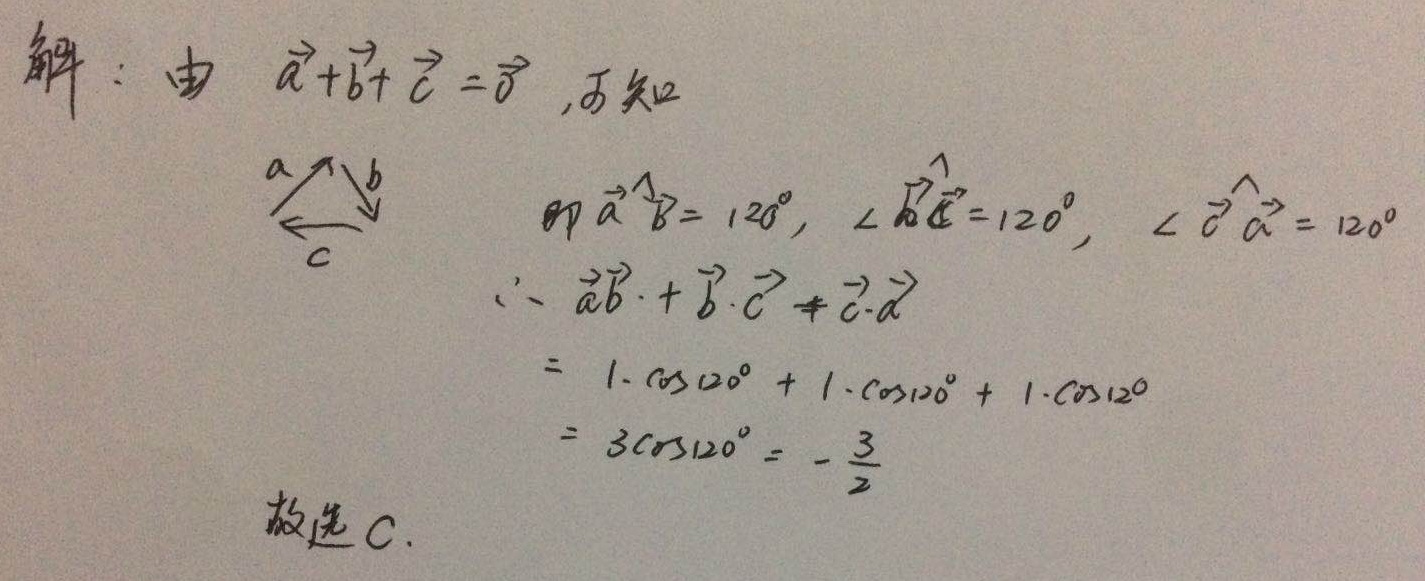
\includegraphics[scale=0.3]{13.jpg}
\subsection{第二周}
\paragraph{ }
1.设点(1,2,3),(-1,0,-6)是某直线上的点,则直线的对称式方程为()
\begin{enumerate}
\item $\frac{x+1}{2}=\frac{y}{2}=\frac{z+6}{9}$\\
\item $\frac{x-1}{2}=\frac{y-2}{2}=\frac{z-3}{3}$\\
\item $\frac{x-2}{2}=\frac{y-2}{2}=\frac{z-9}{9}$\\
\item $\frac{x+1}{1}=\frac{y}{2}=\frac{z+6}{3}$
\end{enumerate}
正确答案A,错选C\\
解:方向向量$\overrightarrow{AB}=(-2,-2,-9)$,取B点,则点向式方程为A

\paragraph{ }
2.设直线的一般式方程为$\left\{
\begin{array}{ll}
x-y+2z-1=0\\
2x+y-z-2=0
\end{array}
\right. 
$,则直线的对称式方程为()
\begin{enumerate}
\item $\frac{x-1}{1}=\frac{y}{-5}=\frac{z}{-3}$\\
\item $\frac{x-1}{1}=\frac{y}{5}=\frac{z+1}{3}$\\
\item $\frac{x-1}{1}=\frac{y}{5}=\frac{z}{3}$\\
\item $\frac{x-1}{1}=\frac{y}{-5}=\frac{z+1}{-3}$
\end{enumerate}
正确答案A,错选D\\
解:方向向量为$\overrightarrow{s}=\overrightarrow{n1}\times\overrightarrow{n2}$,再取点(1,0,0),得点向式方程A。

\paragraph{ }
3.平面$\alpha$分两点A(1,2,3)和B(2,-1,4)间的线段,并垂直。求平面方程为()
\begin{enumerate}
\item $2x-6y+2z-7=0$\\
\item $x-3y+z+2=0$\\
\item $2x-6y+2z+7=0$\\
\item $x-3y+z-12=0$\\
\end{enumerate}
正确答案A,未有任何选项\\
解:设平面与线段AB的交点为p(x,y,z),根据题意$\overrightarrow{AB}//\overrightarrow{Ap}//\overrightarrow{pB},|\overrightarrow{Ap}|=|\overrightarrow{pB}|$,平面的法线是$\overrightarrow{AB}=(1,-3,1)$,关键是求得p点。
根据以上判断可得直线的参数方程$\left\{\begin{array}{ll}
x=t+1\\
y=-3t+2\\
z=t+3
\end{array}
\right.
$,再根据
$|\overrightarrow{Ap}|=|\overrightarrow{pB}|$,可得t=1/2,则可求得
$\left\{ \begin{array}{l}
x=3/2\\
y=1/2\\
z=7/2
\end{array} \right.$,根据点法式方程$A(x-x0)+B(y-y0)+C(z-z0)=0$得到方程为A。
\subsection{第三周}
曲面方程:\\
旋转曲面方程:xoy面$f(x,y)$曲线,绕x轴的曲面方程:$f(x,\sqrt[2]{y^2+z^2})$\\
柱面方程:xoy面,$C:f(x,y)=0$称为准线,平行于z轴的直线l称为母线,由C和l构成的曲面为柱面,方程为$f(x,y)=0$\\
三元二次方程构成的曲面:\\
\begin{tabular}{|l|l|l|l|}
\hline
曲面名称	&
	椭球面	&
	\begin{tabular}{ll}
	抛物面	& \\
		\tabincell{l}{双曲抛物面\\(马鞍面)}	&
		椭球面
	\end{tabular}	&
	\begin{tabular}{ll}
	双曲面	& \\
		单叶 & 
		双叶
	\end{tabular}	\\
	\hline
方程	&
	\tabincell{l}{$\frac{x^2}{a^2}+\frac{y^2}{b^2}+\frac{z^2}{c^2}=1$\\	
		(a,b,c>0)}	&
	\begin{tabular}{ll}
		\tabincell{l}{$\frac{x^2}{2p}+\frac{y^2}{2q}=z$\\p,q异号}&
		\tabincell{l}{$\frac{x^2}{2p}+\frac{y^2}{2q}=z$\\p,q同号}
	\end{tabular}	&
	\begin{tabular}{ll}
		\tabincell{l}{$\frac{x^2}{a^2}+\frac{y^2}{b^2}-\frac{z^2}{c^2}=1$\\2个二次项为正}&
		\tabincell{l}{$-\frac{x^2}{a^2}-\frac{y^2}{b^2}+\frac{z^2}{c^2}=1$\\2个二次项为负}
	\end{tabular}	\\
\hline
曲面图形	&
	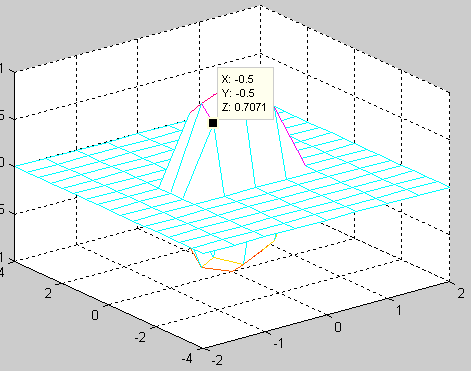
\includegraphics[scale=0.1]{2.png}	&
	\begin{tabular}{ll}
	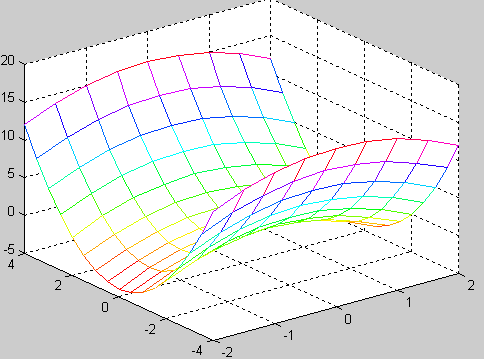
\includegraphics[scale=0.1]{1.png}	&
	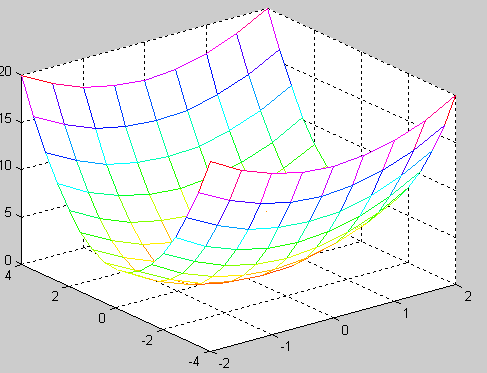
\includegraphics[scale=0.1]{3.png}
	\end{tabular}	&
	\begin{tabular}{ll}
	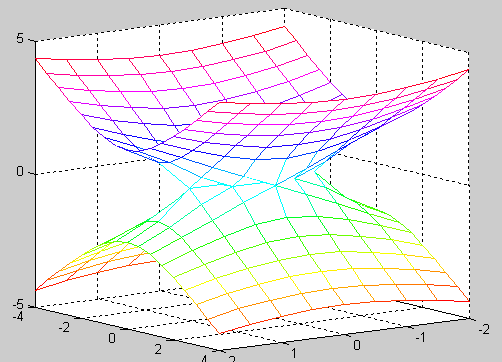
\includegraphics[scale=0.1]{4.png} & 
	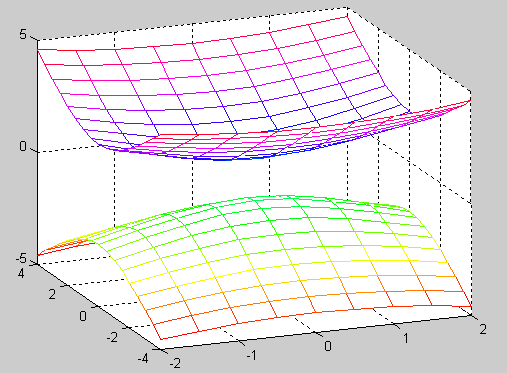
\includegraphics[scale=0.1]{5.png}
\end{tabular}\\
\hline
\end{tabular}\\

\begin{tabular}{|l|l|}
\hline
曲面名称	&
椭圆锥面	\\
\hline
方程	&
	$\frac{x^2}{a^2}+\frac{y^2}{b^2}=z^2$\\
\hline
曲面图形	&
	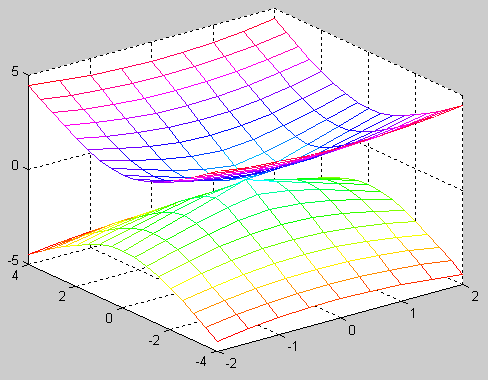
\includegraphics[scale=0.1]{6.png}\\
\hline
\end{tabular}

投影方程:\\
1)消去z变量\\
2)z=0
\paragraph{ }
1.双曲抛物面(马鞍面)$x^2-y^2=2z$与xoy平面的交线是()。
\begin{enumerate}
\item 相交于原点的两条直线.
\item 双曲线
\item 抛物线
\item 椭圆
\end{enumerate}
正确答案A,错选B\\
解:xoy面的方程为z=0,与马鞍面方程联立得到$x=\pm y$,所以答案为A
\paragraph{ }
2.方程$\left \{ \begin{array}{l}
x^2-4y^2+z^2=25\\
x=-3
\end{array} \right.$表示()
\begin{enumerate}
\item x=-3平面上的抛物线
\item 双曲柱面
\item 单叶双曲面
\item x=-3平面上的双曲线
\end{enumerate}
正确答案D,错选为A\\
解:将x=-3带入方程得到的是一个平行于zoy面的平面上的双曲线。如果没有x=-3的条件是双曲柱面,但是这里有x=-3的条件所以只能是一个曲线。
\section{多元函数微分}
\subsection{第四周}
\paragraph
1.$\frac{\partial{f(x,y)}}{\partial{x}}$和$\frac{\partial{f(x,y)}}{\partial{y}}$在点$p(x_0,y_0)$是连续的,是函数f(x,y)在点(x0,y0)可微的()
\begin{enumerate}
	\item 必要条件
	\item 无关条件
	\item 充分条件
	\item 充分必要条件
\end{enumerate}
正确答案C,错选为A
\paragraph
2.设$z=arctan\frac{x+y}{x-y}$,则$\frac{\partial z}{\partial x},\frac{\partial z}{\partial y}$=()
\begin{enumerate}
	\item $\frac{y}{x^2+y^2},\frac{x}{x^2+y^2}$
	\item $-\frac{y}{x^2+y^2},-\frac{x}{x^2+y^2}$
	\item $\frac{y}{x^2+y^2},-\frac{x}{x^2+y^2}$
	\item $-\frac{y}{x^2+y^2},\frac{x}{x^2+y^2}$
\end{enumerate}
正确答案为D,错选为B。
\subsection{第五周}
例1 :设函数$f(x,y,z)=xy^2z^3$,若$y=y(z,x)$为方程$x^2+y^2+z^2-3xyz=0$确定的隐函数,则$f_x(1,1,1)=?$

解: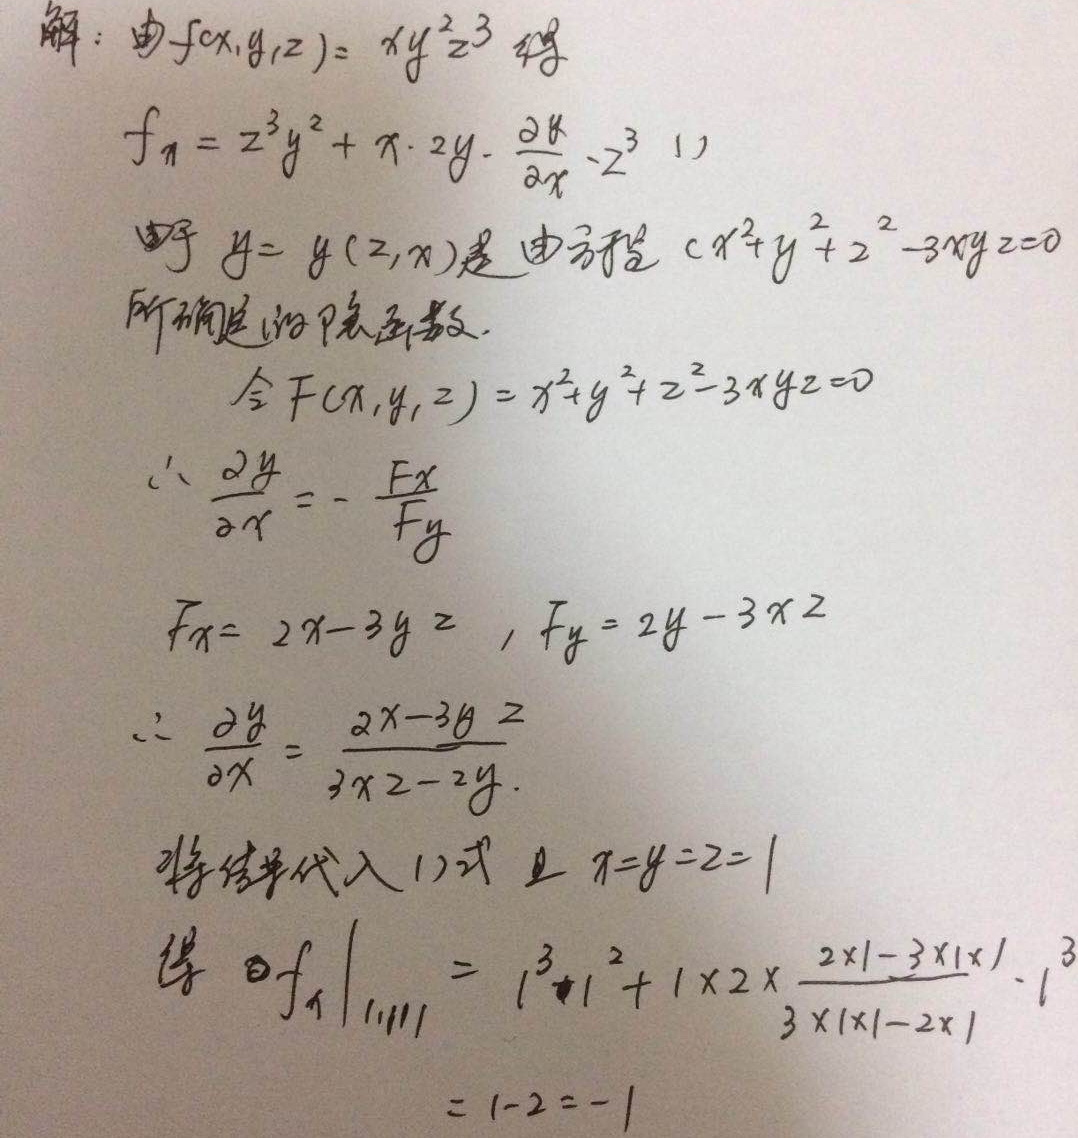
\includegraphics[scale=0.3]{7.jpg}
\subsection{第六周}

1. 下列向量中,与曲线
		\[
			\left \{
				\begin{array}{ll}
					x^2+y^2+z^2-2y=4 \\ 
					x+y+z=0
				\end{array}
			\right. 
		\]
	在点(1,1,-2)处的切向量平行的是()
\begin{enumerate}
	\item (2,-3,1)
	\item (2,-3,-1)
	\item (2,3,1)
	\item (-2,-3,1)
\end{enumerate}
正确答案为A,未有任何选项。

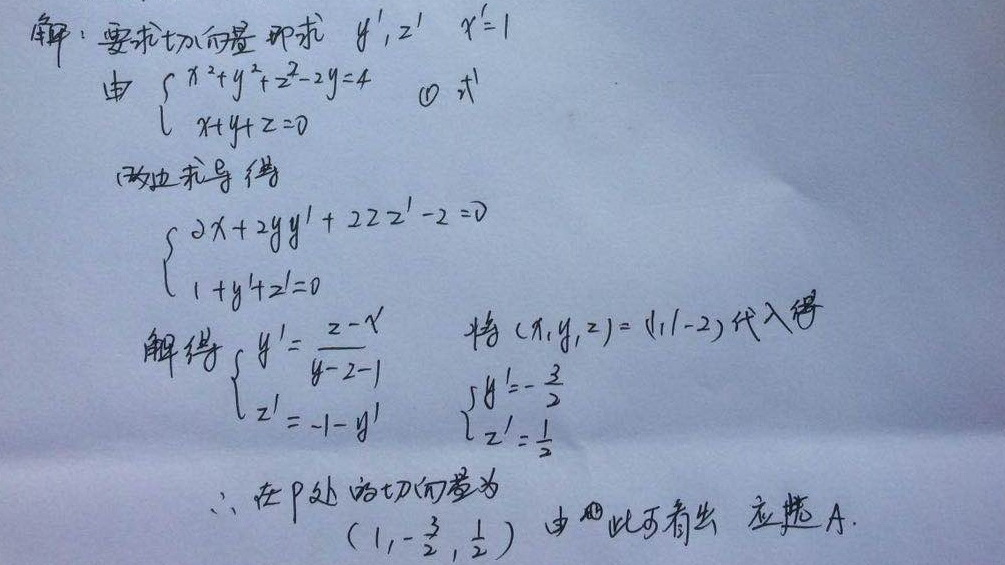
\includegraphics[scale=0.5]{8.jpg}

2. 曲面$z=arcsin\sqrt{1-x^2-y^2}$在点$(0,1/2,\pi/3)$处的切平面的法向量是()
\begin{enumerate}
	\item ($2\sqrt{3}/3,2\sqrt{3}/3,1$)
	\item ($0,,2\sqrt{3},3$)
	\item ($0,2\sqrt{3}/3,-1$)
	\item ($2\sqrt{3}/3,2\sqrt{3}/3,-1$)
\end{enumerate}
正确答案为B,错选为C 

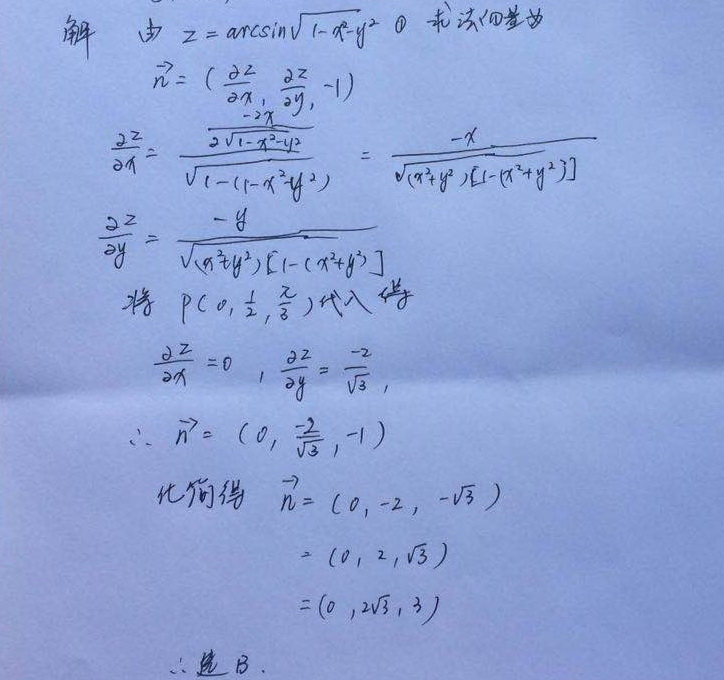
\includegraphics[scale=0.5]{9.jpg}

3. 曲面$z=2x^2+y^2$,该曲面与平面$x+y+z=0$平行的切平面方程为()
\begin{enumerate}
	\item ($x+y+z+3/8=0$)
	\item ($x+y+z+1/8=0$)
	\item ($x+y+z-5/8=0$)
	\item ($x+y+z-9/8=0$)
\end{enumerate}
正确答案为A,错选为D

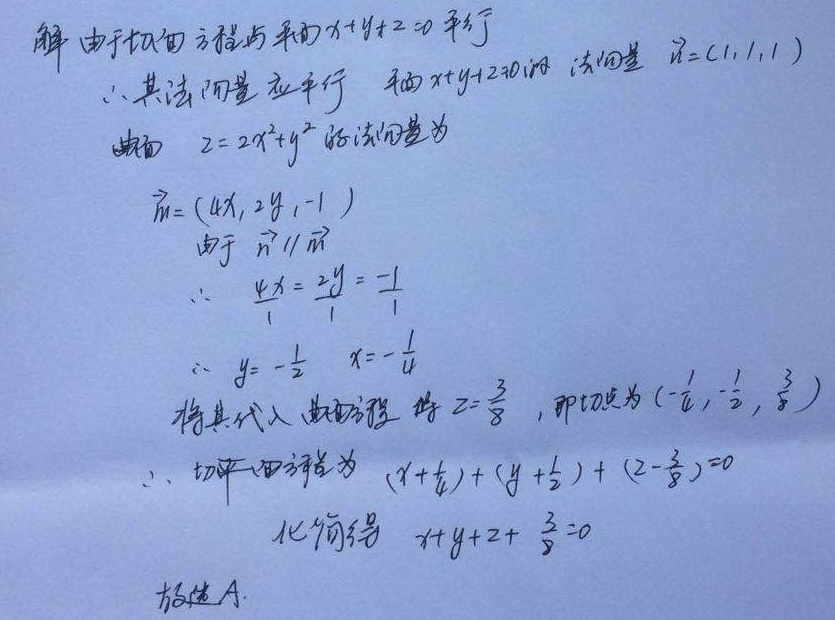
\includegraphics[scale=0.5]{10.jpg}

4. 平面$x+y-z+a=0$是曲面$z=x^2+y^2$的切平面,则a为()
\begin{enumerate}
	\item 2
	\item 1/2
	\item 1
	\item 0
\end{enumerate}
正确答案为B,错选为D

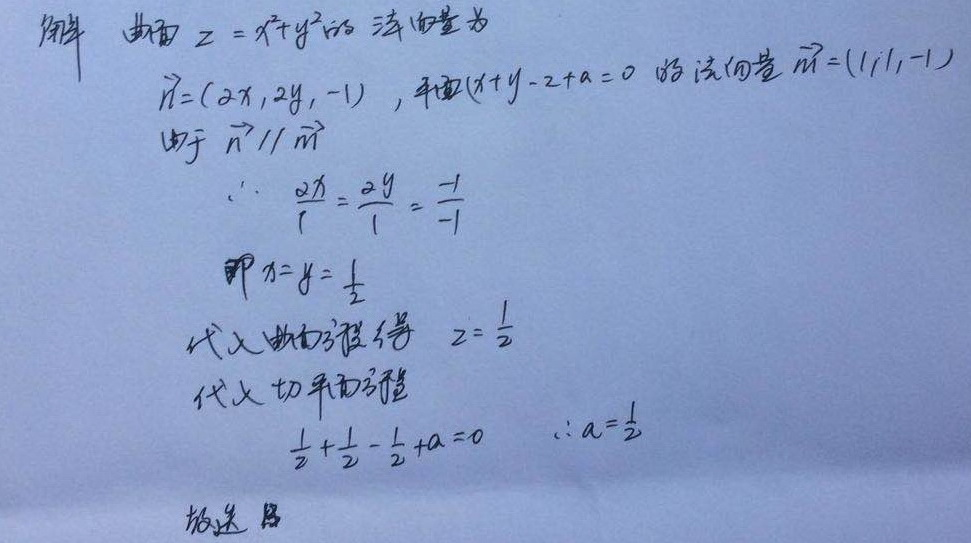
\includegraphics[scale=0.5]{11.jpg}

5. 函数$z=f(x,y)=\sqrt{x^2+y^2}$在点$(0,0)$处函数值增加最快的方向是()
\begin{enumerate}
	\item (1,1)
	\item (1,-1),(-1,1)
	\item (1,1),(-1,-1)
	\item (-1,-1)
\end{enumerate}
正确答案为C,错选为A

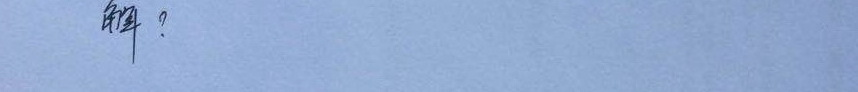
\includegraphics[scale=0.5]{12.jpg}

\section{多元函数积分}
\section{级数}
\newpage
\section{附录1 常用公式}
双曲函数\\
\begin{tabular}{|l|l|l|}
	\hline
	$sh(x)=\frac{e^(x)-e^{-(x)}}{2}$ & 
	$ch(x)=\frac{e^2+e^{-x}}{2}$ & 
	$th(x)=\frac{e^x-e^{-x}}{e^x+e^{-x}}$ \\
	\hline
	$sh'(x)=ch(x)$ &
    $ch'(x)=sh(x)$ & 
	$th'(x)=\frac{1}{ch^2(x)}$\\
	\hline
	$arcsh(x)=ln(x+\sqrt{x^2+1})$ & 
	$arcch(x)=ln(x+\sqrt{x^2-1})$ & 
	\tabincell{l}{$arcth(x)=\frac{1}{2}ln\frac{1+x}{1-x}$\\$x\in(-1,1)$}\\
	\hline
	$arcsh'(x)=\frac{1}{x^2+1}$ &
   $arcch'(x)=\frac{1}{x^2-1} $ &
	$arcth'(x)=\frac{1}{1-x^2}$\\
	\hline 
\end{tabular}\\
$ch^2(x)-sh^2(x)=1$\\
$ch^2(x)+sh^2(x)=ch(2x)$\\
\begin{tabular}{|l|l|}
	\hline
欧拉公式 & $e^{j\theta}=cos\theta+jsin\theta$\\
	\hline
万能公式 & \tabincell{l}{
	$tan\alpha=\frac{2tan(\frac{\alpha}{2})}{1-tan(\frac{\alpha}{2})^2}$\\
	\hline
	$sin\alpha=\frac{2tan(\frac{\alpha}{2})}{1+tan(\frac{\alpha}{2})^2}$\\
	\hline
	$cos\alpha=\frac{1-tan^2(\frac{\alpha}{2})}{1+tan(\frac{\alpha}{2})^2}$\\
}\\
\hline
\end{tabular}
\newpage
\section{附录2不定积分的常用方法} 
	\subsection{基本初等函数积分公式}
		\subsubsection{幂函数}
		\[
			\int x^\mu dx=
			\left \{
				\begin{array}{ll}
					\frac{x^{\mu+1}}{\mu + 1} + C & \mu \neq -1 \\
								 ln|x| + C & \mu =-1
				\end{array}
			\right. 
		\]
		\subsubsection{指数函数}
		$\int e^x dx=e^x+C$\\
		$\int a^x dx=\frac{a^x}{lna}+C$
		\subsubsection{对数函数}
		$\int lnx dx=x*lnx-x+C$\\
		$\int log_a x dx=x*log_a x -xlog_ae+C$
		\subsubsection{三角函数}
			\begin{tabular}{ll}
				$\int sinxdx=cosx+C$ & $\int cosxdx=-sinx+C$\\
				$\int tanxdx=-ln|cosx|+C$ & $\int cotxdx=ln|sinx|+C $\\
				$\int secxdx=ln|secx+tanx|+C $ & $\int cscxdx=ln|cscx-cotx|+C$
			\end{tabular}
		\subsubsection{反三角函数}
			\begin{tabular}{ll}
				$\int arcsinx=x*arcsinxdx+\sqrt{1-x^2}+C$ & $\int arccosxdx=x*arccosx-\sqrt{1-x^2}+C$\\
				$\int arctanxdx=x*arctanx-\frac{1}{2}ln(1+x^2)+C$ & $\int arccotxdx=x*arccotx+\frac{1}{2}ln(1+x^2)+C $\\
				$\int arcsecxdx=x*arcsecx-ln(x+\sqrt{x^2-1})+C $ & $\int arccscxdx=x*arccscx+ln(x+\sqrt{x^2-1})+C$
			\end{tabular}
	\subsection{常用积分公式}
		\begin{tabular}{|l|l|}
			\hline
			$\int \frac{dx}{x^2-a^2}=\frac{1}{2a}ln|\frac{x-a}{x+a}|+C$ & $\int \frac{dx}{x^2+a^2}=\frac{1}{a}arctan\frac{x}{a}+C$\\
			\hline
		$\int \frac{dx}{\sqrt{1-x^2}}=arcsin(x)+C$ & $\int \frac{-dx}{\sqrt{1-x^2}}=arccos(x)+C$\\
			\hline
		 $\int \frac{dx}{1+x^2}=arctan(x)+C$ & $\int \frac{-dx}{1+x^2}=arccot(x)+C$\\
		\hline
		\end{tabular}\\


	\subsection{常用方法}
		1.凑微分\\
		$\int f(\varphi(x))\varphi^{'}(x)dx=\int f(\varphi(x))d(\varphi(x))$\\
		将$\varphi^{'}(x)dx$凑到$d(\varphi(x))$中。\\
		2.换元法\\
		$\int f(x)dx=\int f(\varphi(t))\varphi^{'}(t)dt$\\
		用$x=\varphi(t)$进行替换变量,进行积分\\
		常用换元:\\
		\begin{tabular}{|l|l|}
\hline
			型式 & 换元\\
\hline
			$\sqrt{a^2+x^2}$ & $x=a*tan(\alpha),x=a*sh(\alpha),$\\
			$\sqrt{a^2-x^2}$ & $x=a*sin(\alpha),x=a*cos(\alpha),$\\
			$\sqrt{x^2-a^2}$ & $x=a*sec(\alpha),x=a*csc(\alpha)$,\\
\hline
		\end{tabular}

		3.分部积分\\
		$\int udv=uv-\int vdu$\\
		换一种形式积分
	\subsection{常用形式}
		\subsubsection{含$ax+b$}
		1)采用凑微分方法,将$ax+b$凑到微分中。\\
		2)因式分解\\
		\subsubsection{含$\sqrt{ax+b}$}
		1)利用$t=\sqrt{ax+b}$来去除根号。\\
		2)利用已经获得的结果,分部积分。\\
		参考例子:\\
			$\int \sqrt{ax+b}dx$,凑微分。\\ 
			$\int x\sqrt{ax+b}dx$,利用$t=\sqrt{ax+b}$来去除根号。或分部积分。\\ 
			$\int x^2\sqrt{ax+b}dx$,利用$t=\sqrt{ax+b}$来去除根号。或分部积分。\\ 
			$\int \frac{x}{\sqrt{ax+b}}dx$,利用$t=\sqrt{ax+b}$来去除根号。或先求出$\int \frac{dx}{\sqrt{ax+b}}$,再分部积分。\\ 
			$\int \frac{x^2}{\sqrt{ax+b}}dx$,利用$t=\sqrt{ax+b}$来去除根号。或先求出$\int x/\frac{dx}{\sqrt{ax+b}}$,再分部积分。\\ 
			$\int \frac{dx}{x*\sqrt{ax+b}}$,利用$t=\sqrt{ax+b}$来去除根号,然后利用$\int\frac{dx}{x^2+a^2}=\frac{1}{|a|}arctan(\frac{x}{|a|})+C $和$\int\frac{dx}{x^2-a^2}=\frac{1}{2a}ln(|\frac{x-a}{x+a}|)+C$来积分,。需要根据b>0,b<0选择积分型式。\\ 
			$\int \frac{dx}{x^2*\sqrt{ax+b}}$,需要先分解因式,然后利用$\int \frac{dx}{x*\sqrt{ax+b}}$结果。\\

		\subsubsection{含$a^2 \pm x^2$}	
		\[
		\begin{array}{|l|}
			\hline
			\int\frac{dx}{x^2+a^2}=\frac{1}{|a|}arctan(\frac{x}{|a|})+C\\
			\int\frac{dx}{x^2-a^2}=\frac{1}{2a}ln(|\frac{x-a}{x+a}|)+C \\
			\hline
		\end{array}
		\]
		\subsubsection{含$ax^2+b$}
		1)凑微分\\
		2)分解\\
		参考例子:\\
		\begin{itemize}
			\item	$\int \frac{dx}{ax^2+b}$,利用$\int\frac{dx}{x^2+a^2}=\frac{1}{|a|}arctan(\frac{x}{|a|})+C $和$\int\frac{dx}{x^2-a^2}=\frac{1}{2a}ln(|\frac{x-a}{x+a}|)+C $\\
			\item	$\int \frac{xdx}{ax^2+b}$,凑微分\\
			\item	$\int \frac{x^2dx}{ax^2+b}$,分解\\
			\item	$\int \frac{dx}{x*(ax^2+b)}$,分解\\
			\item	$\int \frac{dx}{x^2*(ax^2+b)}$,分解\\
			\item	$\int \frac{dx}{x^3*(ax^2+b)}$,利用上一个分解的结果分解\\
		\end{itemize}
		\subsubsection{含$ax^2+bx+c,(a>0)$}
		1)凑微分\\
		2)分解\\
		参考例子:\\
		\begin{itemize}
			\item $\int \frac{dx}{ax^2+bx+c}$,\\
			方法1:考虑将$ax^2+bx+c$分解成$(Ax+B)^2+C^2$形式,然后利用$\int\frac{dx}{x^2+a^2}=\frac{1}{|a|}arctan(\frac{x}{|a|})+C $和$\int\frac{dx}{x^2-a^2}=\frac{1}{2a}ln(|\frac{x-a}{x+a}|)+C $。因为$\sqrt{b^2-4ac}$结果不定,所以有两个结果\\
			方法2:由于$\frac{1}{x-r1}*\frac{1}{x-r2}=\frac{1}{r1-r2}(\frac{1}{x-r1}-\frac{1}{x-r2})$,将$ax^2+bx+c$分解成:$\frac{1}{a}\frac{1}{r1-r2}(\frac{1}{x-r1}-\frac{1}{x-r2})$形式,r1,r2是该方程的根。然后凑微分即可积分。
			\item $\int \frac{xdx}{ax^2+bx+c}$,\\
				凑微分,将x凑到dx中。$\frac{x}{ax^2+bx+c}=\frac{ax+b-b}{ax^2+bx+c}$
		\end{itemize}
		\subsubsection{含$\sqrt{x^2+a^2},(a>0)$}
		1)用$x=a*tan\alpha$利用$\sqrt{1+tan^2\alpha}=sec\alpha$换元来脱根号\\
		2)分解\\
		参考例子:\\
		\begin{itemize}
			\item $\int \frac{dx}{\sqrt{x^2+a^2}}=arcsh\frac{x}{a}+C=ln(x+\sqrt{x^2+a^2})+C$.\\
			用$x=a*tan\alpha$利用$\sqrt{1+tan^2\alpha}=sec\alpha$换元来脱根号\\
			利用$\int secx=ln|secx+tanx|+C$公式。注意回带的时候,利用作图来求三角函数值比较方便。
			\item $\int \frac{dx}{\sqrt{x^2+a^2}^3}$.\\
			用$x=a*tan\alpha$利用$\sqrt{1+tan^2\alpha}=sec\alpha$换元来脱根号\\
			注意回带的时候,利用作图来求三角函数值比较方便。
			\item $\int \frac{xdx}{\sqrt{x^2+a^2}}$.\\
			用$x=a*tan\alpha$利用$\sqrt{1+tan^2\alpha}=sec\alpha$换元来脱根号\\
			注意回带的时候,利用作图来求三角函数值比较方便。
			\item $\int \frac{xdx}{\sqrt{x^2+a^2}^3}$.\\
			用$x=a*tan\alpha$利用$\sqrt{1+tan^2\alpha}=sec\alpha$换元来脱根号\\
			注意回带的时候,利用作图来求三角函数值比较方便。
			\item $\int \frac{x^2dx}{\sqrt{x^2+a^2}}$.\\
			方法1:用$x=a*tan\alpha$利用$\sqrt{1+tan^2\alpha}=sec\alpha$换元来脱根号,注意用此方法需要计算$\int sec^3\alpha d\alpha$,在计算的时候会循环,从而求得。\\
			方法2:将分子拆解成$x^2+a^2-a^2$,然后利用现成公式。需要计算$\int \sqrt{x^2+a^2}dx$。注意用此方法需要计算$\int sec^3\alpha d\alpha$,在计算的时候会循环,从而求得。\\
			\item $\int \frac{x^2dx}{\sqrt{x^2+a^2}^3}$.\\
			方法1:用$x=a*tan\alpha$利用$\sqrt{1+tan^2\alpha}=sec\alpha$换元来脱根号\\
			\item $\int \sqrt{x^2+a^2}dx$.\\
			用$x=a*tan\alpha$利用$\sqrt{1+tan^2\alpha}=sec\alpha$换元来脱根号\\
			注意回带的时候,利用作图来求三角函数值比较方便。\\
			\item $\int \sqrt{x^2+a^2}^3dx$\\
			用$x=a*sh\alpha$利用${1+sh^2 \alpha}=ch^2\alpha$换元来脱根号,得到$\int a^4ch^4\alpha d\alpha$,然后积分\\
			\item $\int x\sqrt{x^2+a^2}^3dx$\\
			凑微分\\
			\item $\int x^2\sqrt{x^2+a^2}^3dx$\\
			分部积分?\\
			x在分母\\
			\item $\int \frac{dx}{x\sqrt{x^2+a^2}}$\\
			用$x=a*tan\alpha$利用$\sqrt{1+tan^2\alpha}=sec\alpha$换元来脱根号\\
			\item $\int \frac{dx}{x^2\sqrt{x^2+a^2}}$\\
			用$x=a*tan\alpha$利用$\sqrt{1+tan^2\alpha}=sec\alpha$换元来脱根号,化简得到$\int cot\alpha*csc\alpha d\alpha=csc\alpha$积分形式\\
		\item $\int \frac{\sqrt{x^2+a^2}}{x}dx$\\
			用$x=a*tan\alpha$利用$\sqrt{1+tan^2\alpha}=sec\alpha$换元来脱根号,化简后,分解得到$a\int (\frac{sin\alpha}{1-sin^2\alpha}+\frac{1}{sin\alpha})d\alpha$积分形式\\
		\item $\int \frac{\sqrt{x^2+a^2}}{x^2}dx$\\
			用$x=a*tan\alpha$利用$\sqrt{1+tan^2\alpha}=sec\alpha$换元来脱根号,化简后,分解得到$\int (\frac{1}{cos\alpha}+\frac{cos\alpha}{1-cos^2\alpha})d\alpha$积分形式\\
		\end{itemize}
		\subsubsection{含$\sqrt{x^2-a^2},(a>0)$}
		1)用$x=a*sec\alpha$利用$\sqrt{1+sec^2\alpha}=tan\alpha$换元来脱根号\\
		2)分解\\
		参考例子:\\
		\begin{itemize}
			\item $\int \frac{dx}{\sqrt{x^2-a^2}}=ln|x+\sqrt{x^2-a^2}|+C$\\
			用$x=a*sec\alpha$利用$\sqrt{1+sec^2\alpha}=tan\alpha$换元来脱根号\\
			注意回带的时候,利用作图来求三角函数值比较方便。\\
		\end{itemize}
		\subsubsection{含$\sqrt{a^2-x^2},(a>0)$}
		1)用$x=a*sin\alpha$利用$\sqrt{1-sin^2\alpha}=cos\alpha$换元来脱根号\\
		2)分解\\
		参考例子:\\
		\begin{itemize}
			\item $\int \frac{dx}{\sqrt{a^2-x^2}}=arcsin(x/a)+C$\\
			直接套用公式,凑微分;或者令$x=asin\alpha$来脱根号。\\
			注意回带的时候,利用作图来求三角函数值比较方便。\\
		\end{itemize}
	\subsubsection{含$\sqrt{\pm ax^2+bx+c},(a>0)$}
		1)凑微分\\
		2)分解\\
		参考例子:\\
		\begin{itemize}
			\item $\int \frac{dx}{\sqrt{ax^2+bx+c}}=\frac{1}{\sqrt{a}}ln|2ax+b+2\sqrt{a}\sqrt{ax^2+bx+c}|+C,a>0$ \\
				将$ax^2+bx+c$分解成$\frac{1}{4a}[(2ax+b)^2+4ac-b^2]=\frac{1}{4a}[(2ax+b)^2-(\sqrt{b^2-4ac})^2]$,然后利用$\int \frac{dx}{\sqrt{x^2-a^2}}$公式积分。

			\item $\int \frac{dx}{\sqrt{-ax^2+bx+c}}=\frac{1}{\sqrt{a}}arcsin(\frac{2ax-b}{\sqrt{b^2+4ac}})+C,a>0$ \\
				将$-ax^2+bx+c$分解成$\frac{1}{4a}[-(2ax+b)^2+4ac+b^2]=\frac{1}{4a}[-(2ax+b)^2+(\sqrt{b^2+4ac})^2]$,然后利用$\int \frac{dx}{\sqrt{a^2-x^2}}$公式积分。
		\end{itemize}
		\subsubsection{含$\sqrt{\pm \frac{x-a}{x+a}}$或$\sqrt{(x-a)(x-b)}$}
		1)$t=\sqrt{\frac{x-a}{x+a}}$,变量代换去根号\\
		参考例子:\\
		\begin{itemize}
			\item $\int \sqrt{\frac{x-a}{x-b}}dx$\\
				两次代换,第一次$t=\sqrt{\frac{x-a}{x+a}}$,第二次$t=seck$


		\end{itemize}
		\subsubsection{含三角函数}
\end{flushleft}
\end{document}

